\problem{}
The processed image by the median filter is shown in Figure \ref{fig:p3a}.

And we could see that the median kernel with size $3 \times 3$ has the best performance in this case.\\
The kernel has the proper size that remove the salt and pepper noise.

From the result, we could see that all the median filter processed images eliminate the salt and pepper noise, but the kernel size $3 \times 3$ has the best performance. The kernel size $5 \times 5$ and $7 \times 7$ make the 
processed images much blur than the $3 \times 3$ kernel size.

Analyse:


\begin{figure}[htbp]
    \centering
	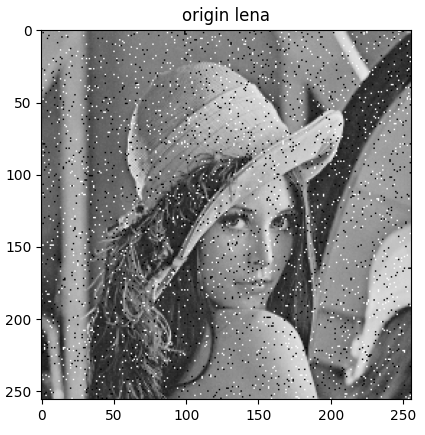
\includegraphics[width=0.48\textwidth]{../images/p3/p3_noisy.png}
	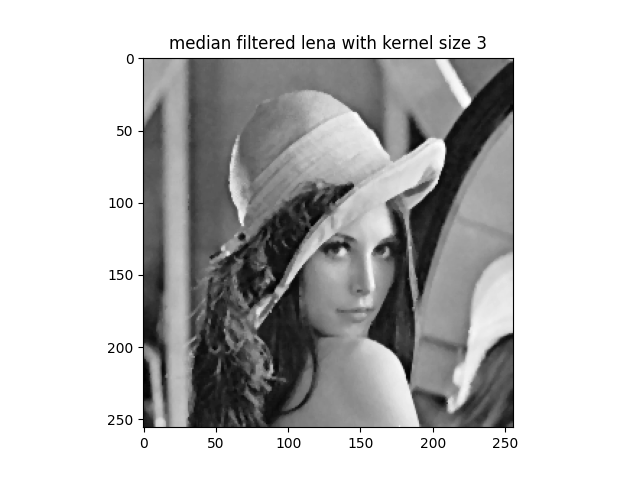
\includegraphics[width=0.48\textwidth]{../images/p3/p3a_3x3.png}
	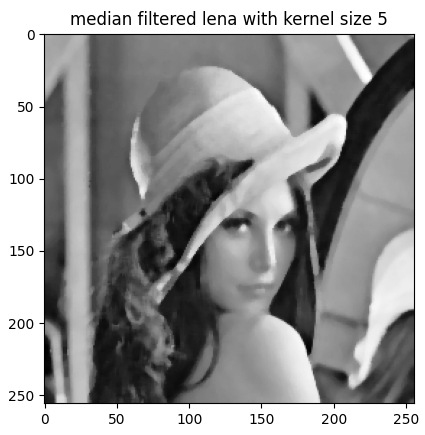
\includegraphics[width=0.48\textwidth]{../images/p3/p3a_5x5.png}
	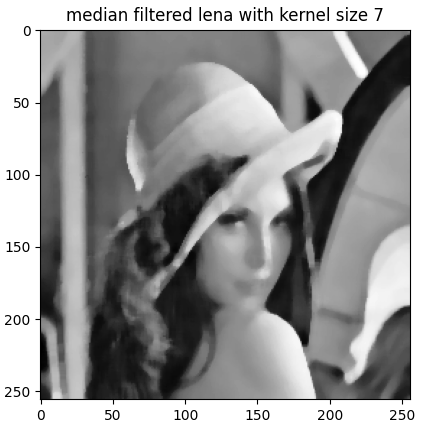
\includegraphics[width=0.48\textwidth]{../images/p3/p3a_7x7.png}
    \caption{Median filter processed image}
\label{fig:p3a}
\end{figure}

The processed image by the and Gaussian filter is shown in Figure \ref{fig:p3b}.

Since the Gaussian filter's elements are $G(s,t)=Ke^{-\frac{s^2+t^2}{2\sigma^2}}$, but with the the normalize factor, the value of
$K$ would be eliminate, so $K$ does not matter. So we can just take $K=1$ and adjust the kernel size.

Analyse:


\begin{figure}[htbp]
    \centering
	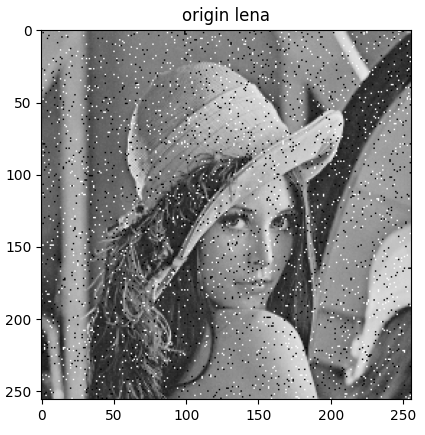
\includegraphics[width=0.48\textwidth]{../images/p3/p3_noisy.png}
	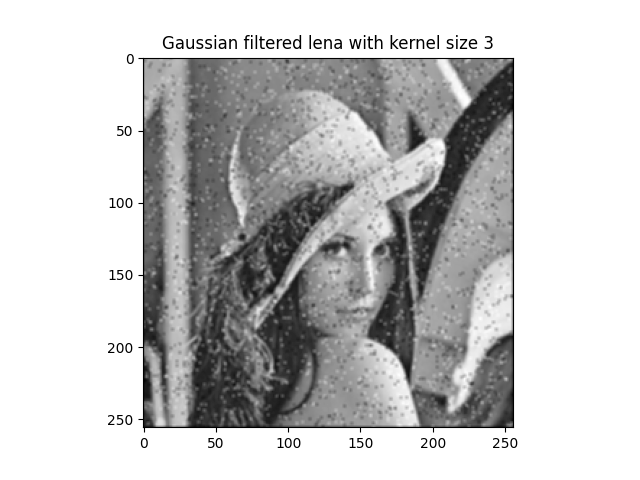
\includegraphics[width=0.48\textwidth]{../images/p3/p3b_3x3.png}
	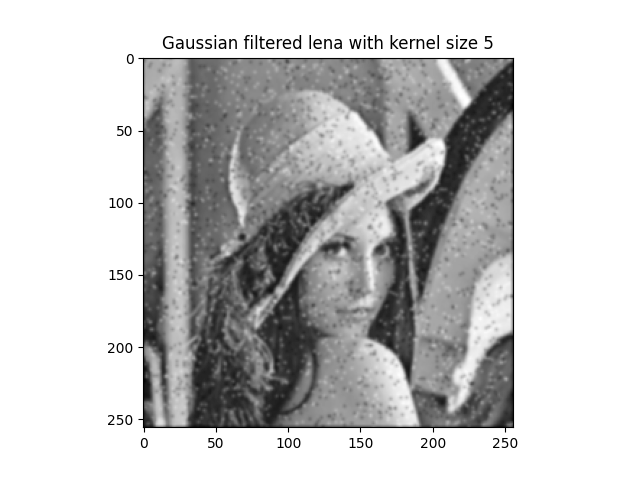
\includegraphics[width=0.48\textwidth]{../images/p3/p3b_5x5.png}
	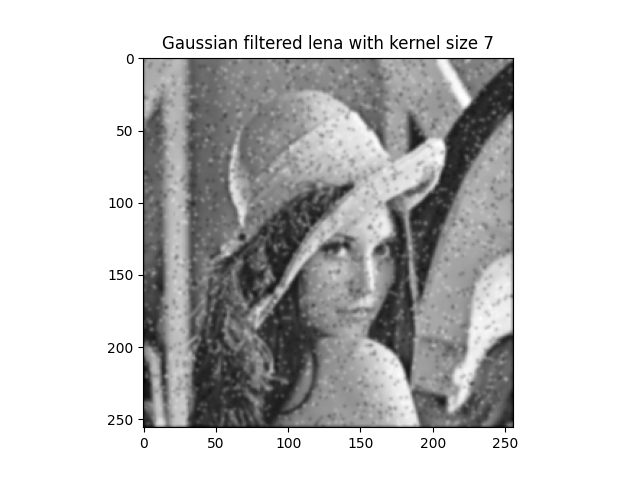
\includegraphics[width=0.48\textwidth]{../images/p3/p3b_7x7.png}
    \caption{Gaussian filter processed image}
\label{fig:p3b}
\end{figure}



Salt-and-pepper noise is a common type of image noise characterized by random occurrences of black (pepper) and white (salt) pixels scattered across an image. When dealing with images afflicted by salt-and-pepper noise, median filters and Gaussian filters are two commonly used denoising methods. Each has its characteristics and is suitable for different denoising needs.
Median Filter
Principle: The median filter works by replacing each pixel value with the median value of all pixel values in its neighborhood. This method is particularly effective for removing salt-and-pepper noise since such noise usually consists of extreme values, and the median filter can preserve image edges well.
Different Sizes of Median Filters:
Small-size filters (e.g., 3x3) can effectively remove noise while preserving the sharpness and details of the image. However, for images with a high density of noise, small-size filters may not be sufficient to completely eliminate the noise.
Large-size filters (e.g., 5x5 or larger) are more effective for images with a high noise density because they provide a larger neighborhood for calculating the median. However, using large-size filters may lead to a loss of image detail, making the image appear blurry.
Gaussian Filter
Principle: The Gaussian filter is a linear smoothing filter that replaces each pixel value with a weighted average of its neighboring pixel values, where the weights are determined by a Gaussian function. This gives the greatest weight to the central pixel, with the weight decreasing as the distance from the central pixel increases.
Different Sizes of Gaussian Filters:
Small-size filters (e.g., 3x3) provide a slight smoothing effect that can remove minor noise while maintaining the overall clarity of the image. However, it may not be very effective at removing salt-and-pepper noise, especially at higher noise levels.
Large-size filters (e.g., 5x5 or larger) provide a stronger smoothing effect, more suitable for removing larger areas of noise. However, this comes at the cost of sacrificing image clarity and detail.
Summary
Removing Salt-and-Pepper Noise: Median filters are generally more suited for removing salt-and-pepper noise than Gaussian filters, especially when the noise density is high.
Preserving Edges: Compared to Gaussian filters, median filters are better at preserving image edges while removing noise.
Filter Size Selection: The size of the filter should be chosen based on the density of the noise and the need to preserve image details. Larger filter sizes, although more effective at noise removal, may also lead to a loss of image detail.
In practical applications, the choice of which filter to use and what size to employ often depends on the specific characteristics of the image and denoising requirements, which may need to be determined through experimentation to find the optimal settings.